% Created 2024-10-16 śro 21:35
% Intended LaTeX compiler: pdflatex
\documentclass[../main.tex]{subfiles}

% \usepackage[a4paper, margin=3cm]{geometry}
% \usepackage{amssymb} // not working

\usepackage[T1]{fontenc}
\usepackage[utf8]{inputenc}
\usepackage{graphicx}
\usepackage{longtable}
\usepackage{wrapfig}
\usepackage{rotating}
\usepackage[normalem]{ulem}
\usepackage{amsmath}
\usepackage{capt-of}
\usepackage{hyperref}
\usepackage{siunitx}
\usepackage{float}
\usepackage[polish]{babel}

\graphicspath{{../}}
\author{Wojciech Paderewski}
\date{\today}
\title{montaz}
\hypersetup{
 pdfauthor={Wojciech Paderewski},
 pdftitle={montaz},
 pdfkeywords={},
 pdfsubject={},
 pdflang={Polish}}

\begin{document}
\subsection{Projekt płytki drukowanej}
Do zaprojektowania płytki drukowanej wykorzystano open-source'owy program KiCad. Zdecydowano się na zastosowanie dwustronnej płytki drukowanej.
Ostatecznie udało się uzyskać płytkę o wymiarach 138x53mm oraz szacowana wysokość wraz z komponentami na poziomie 1cm, 
co oznacza, że udało się osiągnąć cel wykonania jak najmniejszej płytki drukowanej.

W celu poprawy aspektów wizualnych płytki, zamówiona została pozłacana płyta drukowana. Uzyskano też pozłacaną ramkę, która powstała przez 
nie nakładanie soldermaski na krawędzie płytki, w taki sam sposób uzyskano pozłacane napisy. Płytka posiada 4 otwory montażowe ma śruby M3.
Otwory montażowe oraz otwory montażowe encodera są podłączone do masy, co pozwala na lepsze prowadzenie masy między warstwami płytki. W 
celu poprawy uzyskania jak najlepszego połączenia masy między warstwami, użyto dużo przelotek między warstwami. Zabieg ten pozwala na
lepsze ekranowanie ścieżek co powinno przyczynić się do zmniejszenia zakłóceń elektromagnetycznych. 

\begin{figure}[H]
    \centering
    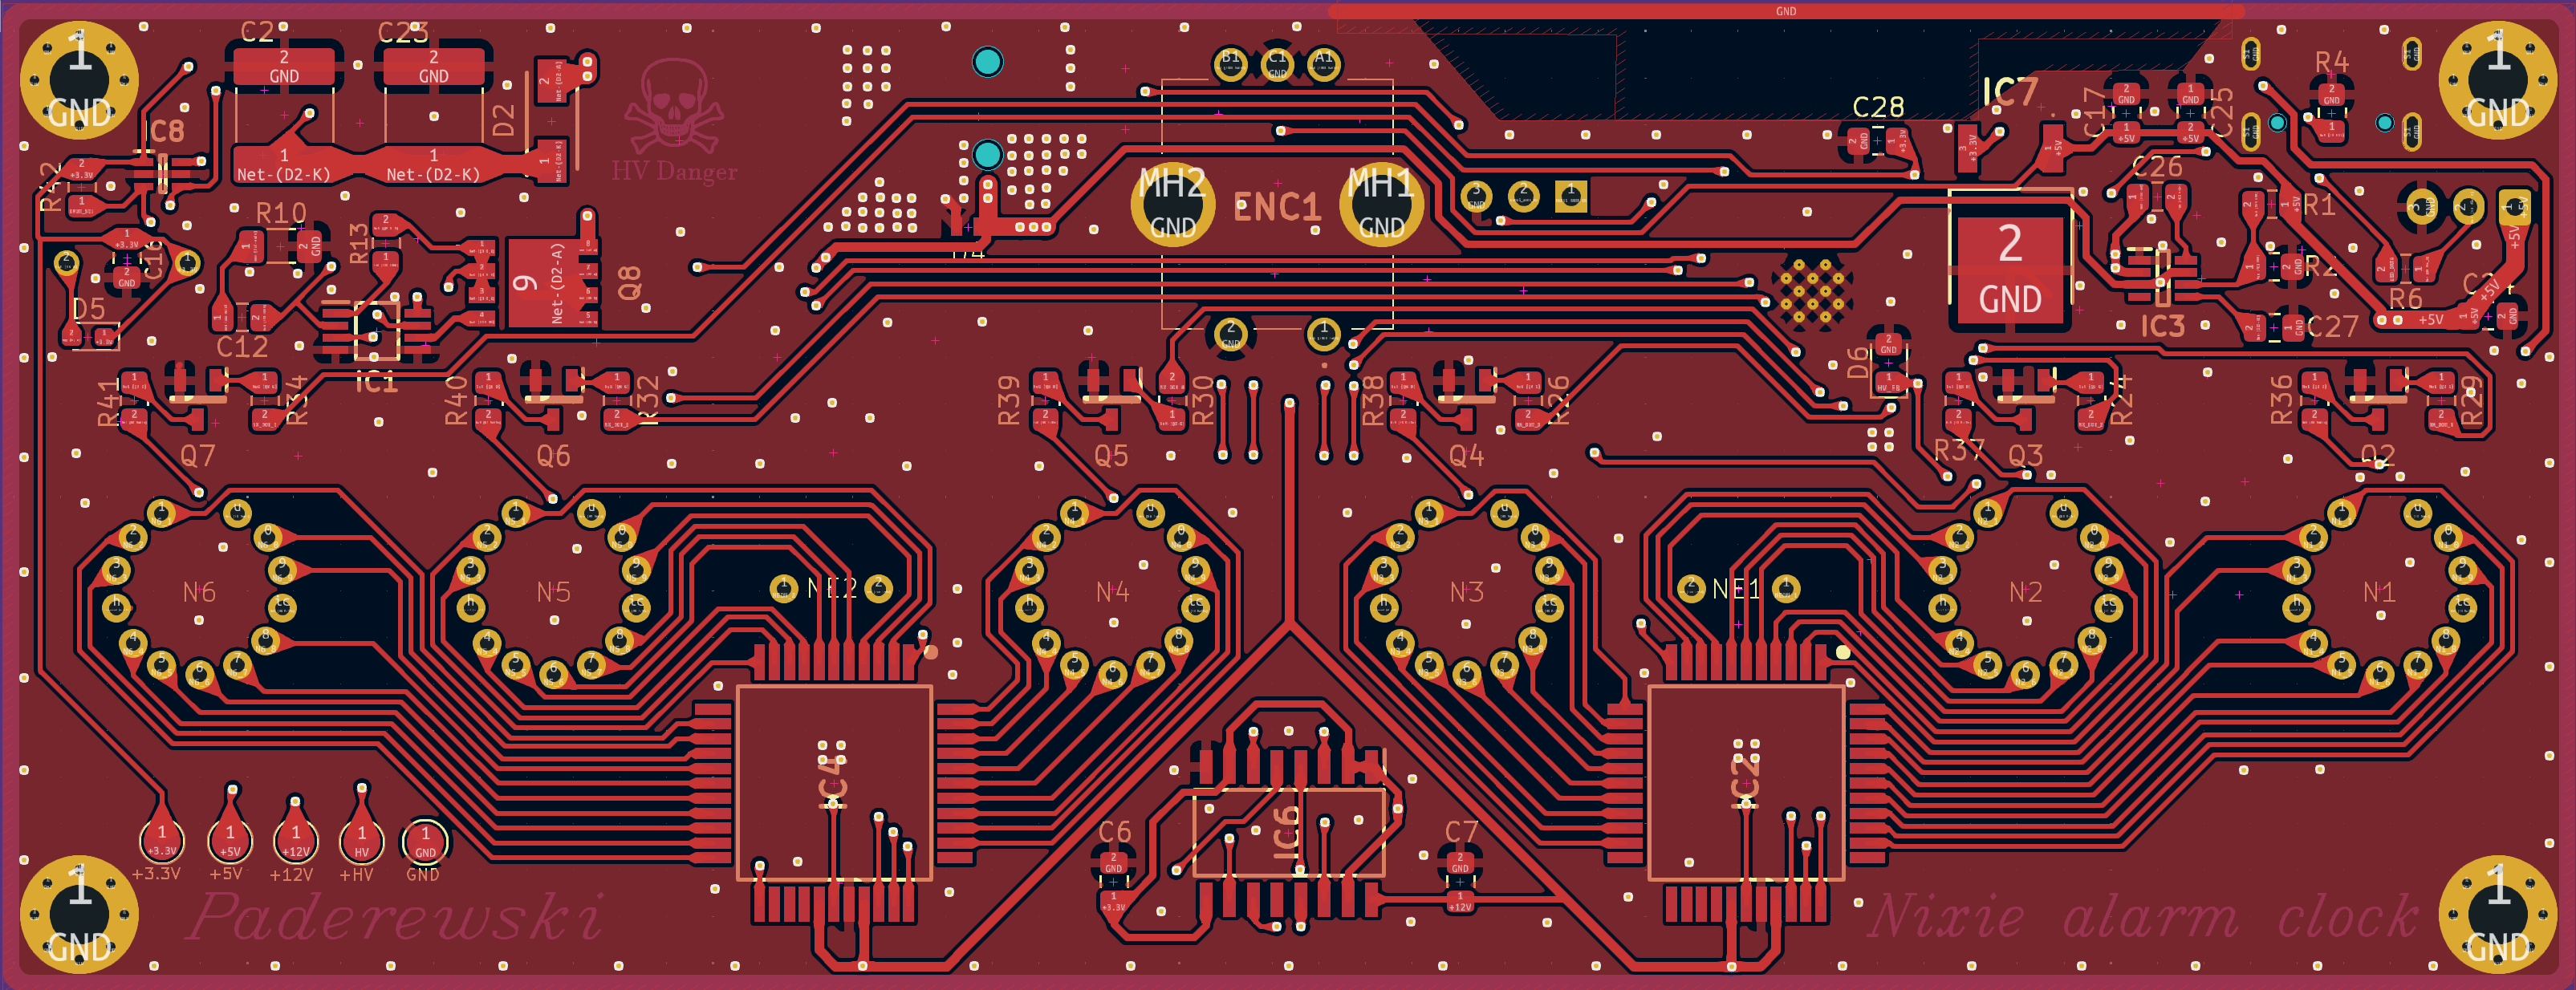
\includegraphics[width=1\textwidth]{TOP.png}
    \caption{Górna warstwa płytki drukowanej}
\end{figure}

\begin{figure}[H]
    \centering
    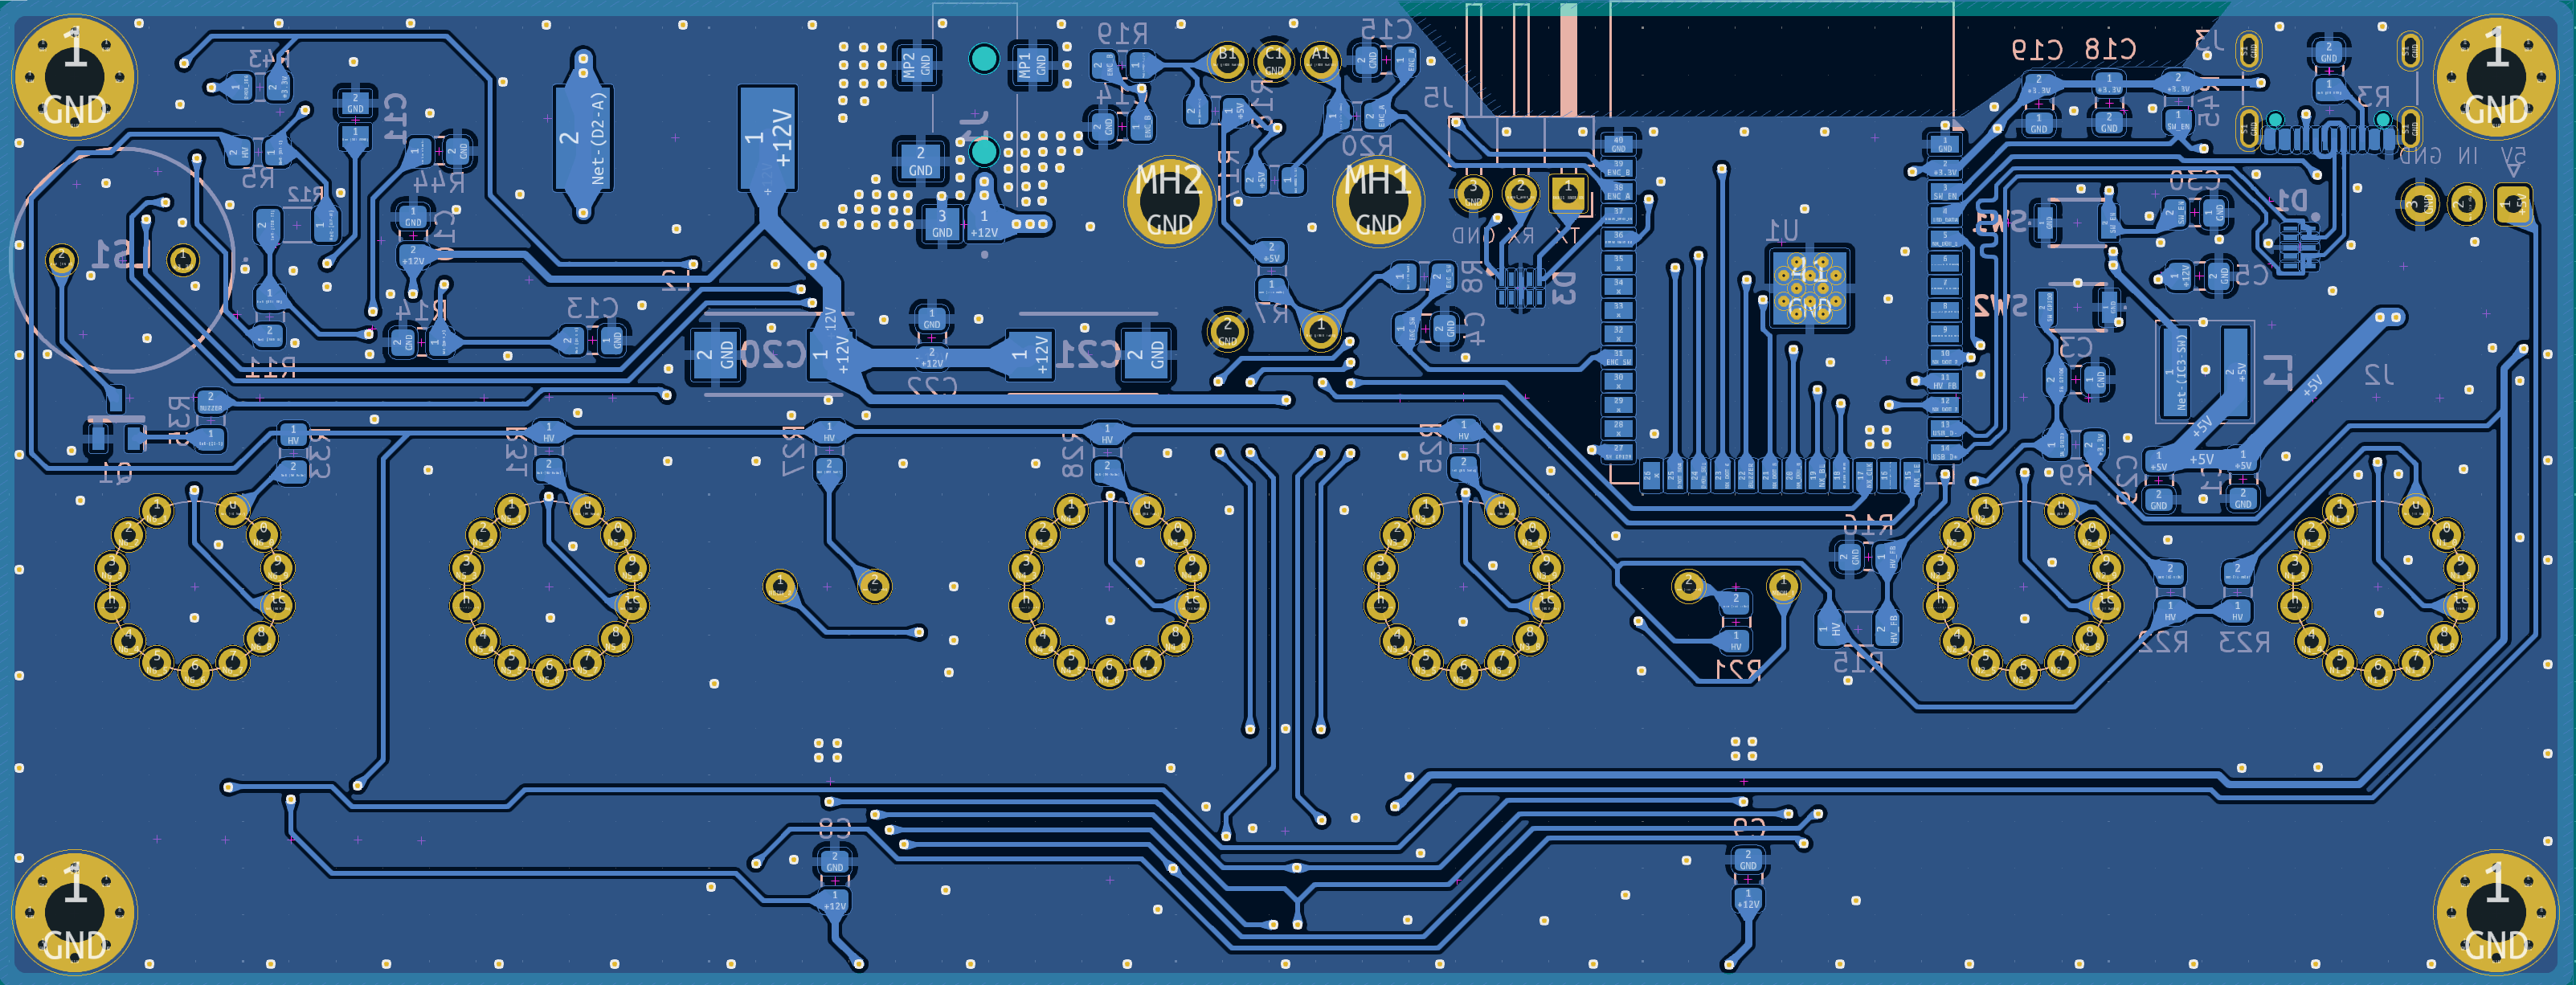
\includegraphics[width=1\textwidth]{BOTTOM.png}
    \caption{Dolna warstwa płytki drukowanej}
\end{figure}

\subsection{Montaż i uruchomienie układu}
Kolejnym etapem realizacji projektu był montaż elementów na płytce drukowanej. Zamówione płytki widzimy na rysunkch \ref{fig:plytka_drukowana_1} oraz \ref{fig:plytka_drukowana_2}.
Przed rozpoczęciem lutowania wszytkie pozłacane elementy
które ostały dodane jak elemnet estetyczny, zostały zabezpieczone przed przypadkowym kontaktem z cyną, w wypadku gdyby cyna dostała się
na pozłacane elementy, nie udałoby się jej usunąć. Do zabezpieczenia wykorzystano taśmę kaptonową, która jest odporna na wysokie temperatury.

\begin{figure}[H]
    \centering
    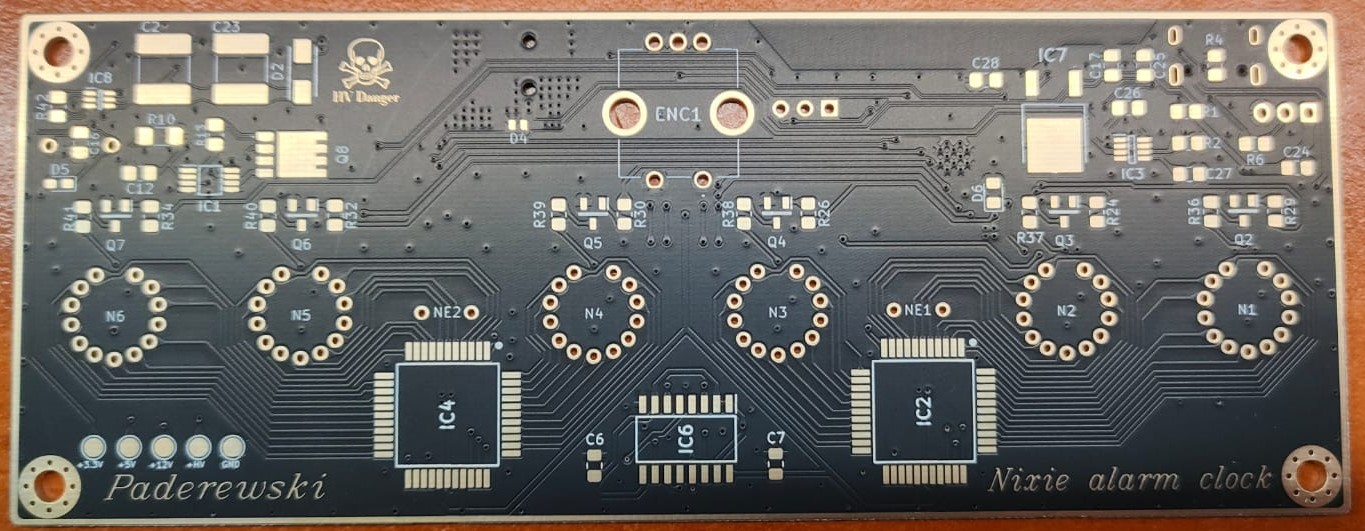
\includegraphics[width=0.85\textwidth]{przod.jpeg}
    \caption{Płytka drukowana - widok od góry}
    \label{fig:plytka_drukowana_1}
\end{figure}

\begin{figure}[H]
    \centering
    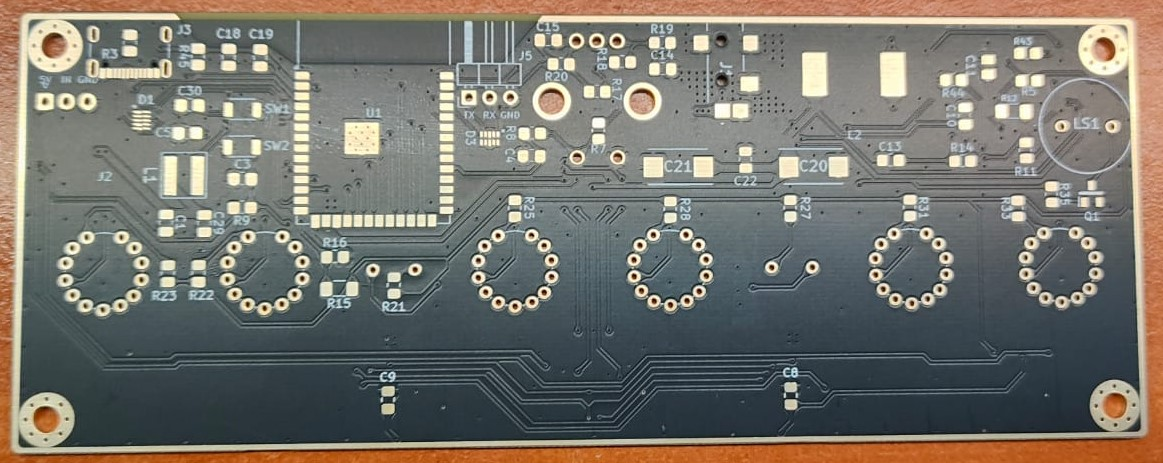
\includegraphics[width=0.85\textwidth]{tyl.jpeg}
    \caption{Płytka drukowana - widok od spodu}
    \label{fig:plytka_drukowana_2}
\end{figure}


Lutowanie rozpoczęto od elementów najmniejszych SMD(montaż powierzchniowy). W celu łatwego lutowania elementów SMD, użyto pasty lutowniczej(flux)
oraz stacji lutowniczej na gorące powietrze(hot air). Po zlutowaniu elementów SMD, wyczyszczono płytkę z nadmiaru topnika, korzystającą z alkoholu izopropylowego. Następnym
krokiem było lutowanie elementów przewlekanych(THT). Ostatnim  mocowanym elementem były lampy Nixie, które trzeba było odpowiednio wypoziomować, by wszystkie lampy
były na tej samej linie. Lampy mają duże tolerancje produkcyjne, co powoduje że niektóre z lamp mogą być wyżej lub niżej niż pozostałe. W celu wypoziomowania lamp,
wykorzystano kątownik. Ostatnim etapem montażu było końcowe czyszczenie płytki z nadmiaru topnika. 

\begin{figure}[H]
    \centering
    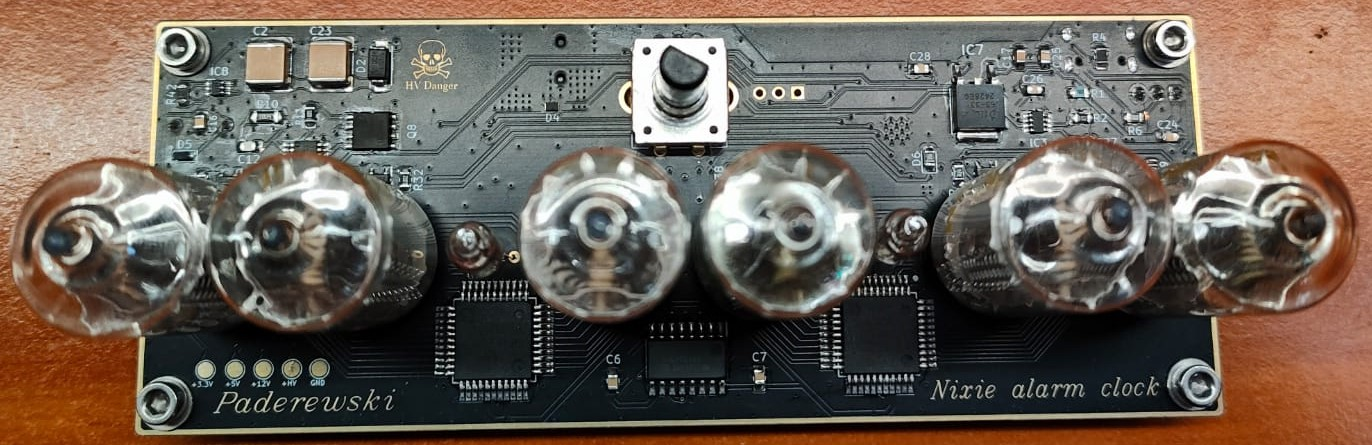
\includegraphics[width=0.85\textwidth]{gora.jpeg}
    \caption{Zmontowana płytka drukowana - widok od góry}
\end{figure}

\begin{figure}[H]
    \centering
    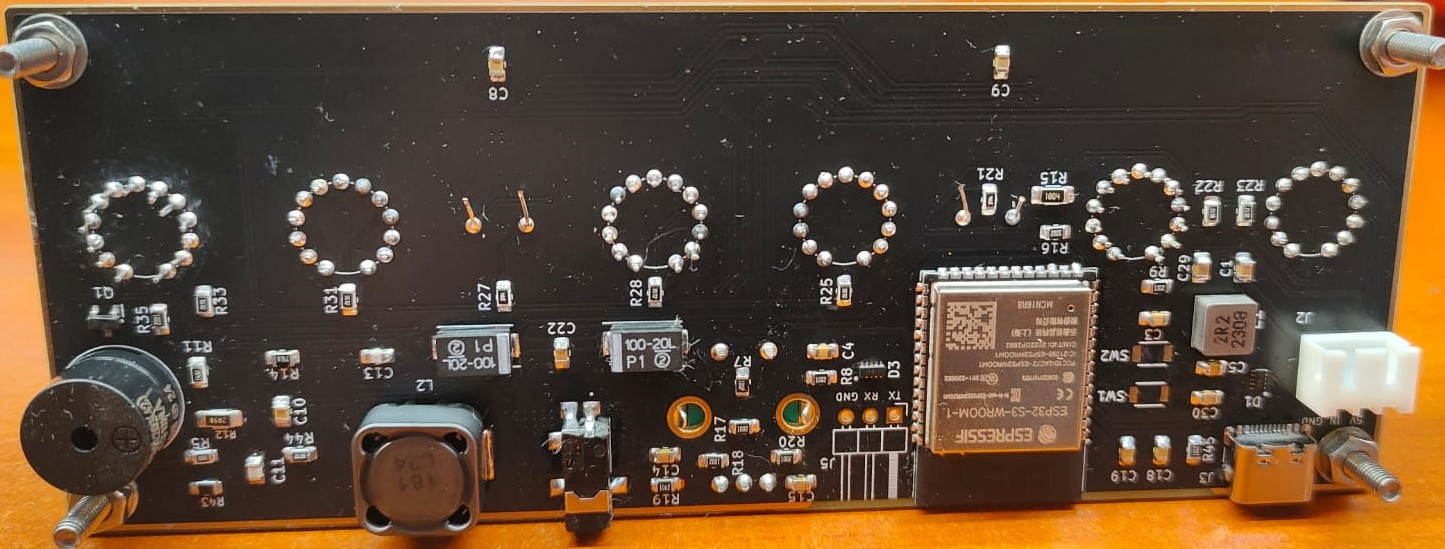
\includegraphics[width=0.85\textwidth]{dol.jpeg}
    \caption{Zmontowana płytka drukowana - widok od spodu}
\end{figure}


\subsection{Uruchomienie układu}
Przetwornica HV jako najtrudniejszy moduł układu, została odizolowana na etap pierwszego uruchomiania, w celu zminimalizowania ryzyka uszkodzenia lamp Nixie. Zrealizowano izolacje
poprzez nie przylutowanie rezystora 0\si{\ohm} na linii łączącej przetwornicę z lampami Nixie. 

Przed podłączeniem zasilania, sprawdzono czy nie ma zwarcia na żadnej linii zasilania.
Po podłączeniu zasilania, sprawdzono napięcia na każdej z sekcji zasilania. Pomierzone napięcia były następujące:
\begin{itemize}
    \item linia 5V - 5.081V
    \item linia 3.3V - 3.306V
    \item linia 12V - 12.01V
    \item linia Wysokie napięcie - 162.1V
\end{itemize}

Wszystkie napięcia są zgodne z wartościami oczekiwanymi. Napięcia są stabilne i nie obserwuje się żadnych skoków napięcia.
Ostatnim krokiem było dolutowanie rezystora 0\si{\ohm} łączącego przetwornicę z lampami Nixie. Na \ref{fig:zmontowany_uklad} został przedstawiony zmontowany układ.

\begin{figure}[H]
    \centering
    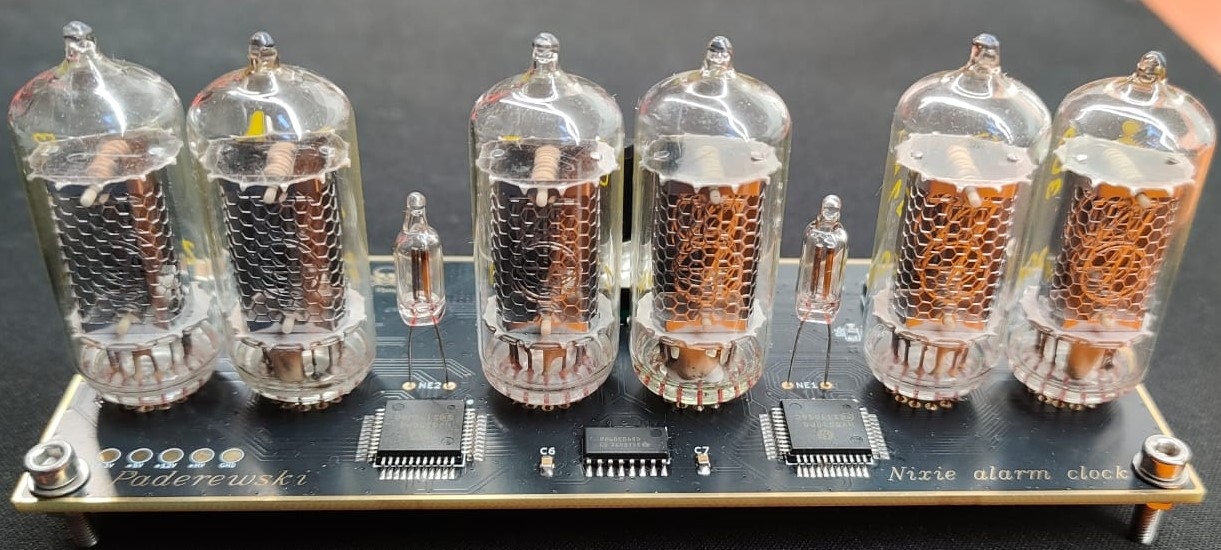
\includegraphics[width=0.85\textwidth]{gotowy.jpeg}
    \caption{Zmontowany układ}
    \label{fig:zmontowany_uklad}
\end{figure}

\end{document}


